\documentclass[tikz,border=5mm]{standalone}
\usepackage{tikz}
\usetikzlibrary{arrows.meta, angles, quotes}
\usetikzlibrary{calc}

\begin{document}
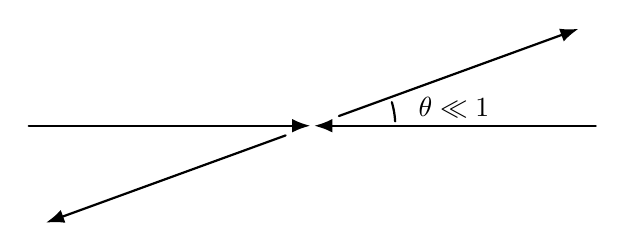
\begin{tikzpicture}[line cap=round, line join=round, >=Latex, scale=1.2]

  % ===== Parameters =====
  \def\L{3}      % length of outgoing rays
  \def\angDeg{20}   % angle (in degrees) above the horizontal for the tilted outgoing line

  % ===== Vertex =====
  \coordinate (O) at (0,0);

  \def\gapA{0.02}   % size of central gap
  \def\gapB{0.3}   % size of central gap

  % Horizontal line (right)
  \draw[<-, thick] ($(O)+(0:\gapA)$) -- ($(O)+(0:\L)$);

  % Horizontal line (left)
  \draw[->, thick] ($(O)+(180:\L)$) -- ($(O)+(180:\gapA)$);

  % Tilted line (right)
  \draw[->, thick] ($(O)+(\angDeg:\gapB)$) -- ($(O)+(\angDeg:\L)$);

  % Tilted line (left)
  \draw[<-, thick] ($(O)+(\angDeg+180:\L)$) -- ($(O)+(\angDeg+180:\gapB)$);
  
  % ===== Angle arc and label between the two outgoing rays =====
  % Define points one unit along each outgoing direction for the angle pic:
  \path (O) -- ++(3:1) coordinate (H)
            -- ++(30:1) coordinate (U);

  % Draw the angle at O between horizontal (H) and tilted (U), label it \theta
  \pic[draw, thick, angle eccentricity=1.8, angle radius=30pt]
      {angle = H--O--U};

  \node[scale=1] at (1.5,0.19) {$\theta \ll 1$};

\end{tikzpicture}

\end{document}
